% migrate-to: portfolio-construction-risk
\section{Overview of Systematic Investments}

A schematic of a live 'production' trading strategy is shown below, but does not include everything else necessary to create the strategy (i.e., research tools).

\begin{figure}[H]
\centering
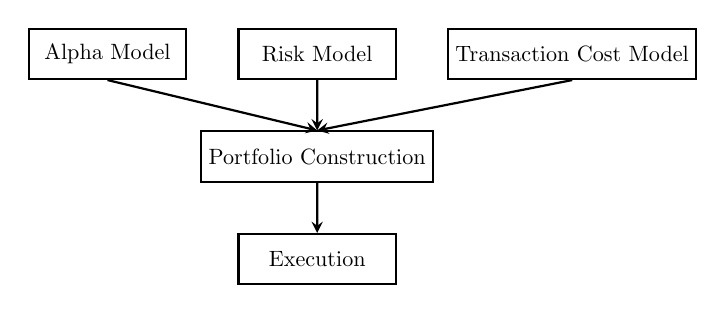
\begin{tikzpicture}[auto, thick, >=stealth, scale=0.8, transform shape]

    \usetikzlibrary{positioning}

    % Three modules arranged horizontally with reduced dimensions
    \node[draw, rectangle, minimum width=2.5cm, minimum height=0.8cm] (alpha) {Alpha Model};
    \node[draw, rectangle, minimum width=2.5cm, minimum height=0.8cm, right=0.8cm of alpha] (risk) {Risk Model};
    \node[draw, rectangle, minimum width=2.5cm, minimum height=0.8cm, right=0.8cm of risk] (tc) {Transaction Cost Model};

    % Portfolio Construction node directly below Risk Model
    \node[draw, rectangle, minimum width=2.5cm, minimum height=0.8cm, below=0.8cm of risk] (portfolio) {Portfolio Construction};

    % Execution node below Portfolio Construction
    \node[draw, rectangle, minimum width=2.5cm, minimum height=0.8cm, below=0.8cm of portfolio] (execution) {Execution};

    % Arrows connecting the nodes
    \draw[->] (alpha.south) -- (portfolio.north);
    \draw[->] (risk.south) -- (portfolio.north);
    \draw[->] (tc.south) -- (portfolio.north);
    \draw[->] (portfolio.south) -- (execution.north);
    
\end{tikzpicture}



\caption{Live Production Trading Strategy Overview}
\end{figure}

At its core, the trading system is organised into three primary modules:

The trading system has three modules:
\begin{enumerate}[label=\roman*.]
	\item Alpha model: predicts the future of the instruments considered for trading, i.e. directional alpha
	\item Risk model: limits amount of exposure to factors that are unlikely to generate returns but could drive losses, i.e. directional exposure limit on an asset class
	\item Transaction cost model: determine if the cost of the trades needed to migrate from current portfolio to new portfolio is desirable to the portfolio construction model.
\end{enumerate}
These models feed into a portfolio construction model that balances the tradeoffs of profit and risk to determine the best portfolio to hold. The model finds the differences in trades that need to be executed.\\
The execution model then takes the required trades, and using inputs such as urgency in which the trades need to be executed and dynamics of liquidity in the markets, executes the trades in an efficient and low cost manner.\\

\begin{method} \hlt{Chains of Production for Alpha Signals}
\begin{enumerate}[label=\roman*.]
\setlength{\itemsep}{0pt}
\item Data Curation: for collecting, cleaning, indexing, storing, adjusting, and delivering all data to production chain. Requires experts in market microstructure and data protocols such as FIX.
\item Feature Analysis: transform raw data into informative signals. Requires experts in information theory, signal extraction and processing, visualisation, labelling, weighting, classifiers, feature importance techniques. Feature analysts collect and catalogue libraries of findings.
\item Strategists: informative features are transformed into actual investment algorithms. Strategists will parse libraries of features for ideas to develop an investment strategy. Require data scientists with deep knowledge of financial markets and economy. Features may be discovered by black box, but strategy is developed in a white box.
\item Back-testers: assess profitability of investment strategy under various scenarios. Requires data scientists with deep understanding of empirical and experimental techniques. Good back-tested incorporates in analysis meta-information on how strategy was created.
\item Deployment Team: integrate strategy code into production line. Requires algorithm specialists and mathematical programmers. To ensure deployed solution is logically identical to prototype, and to optimise implementation sufficiently such that production latency is minimised.
\item Portfolio Oversight: once strategy is deployed, follows lifecycle.
\begin{enumerate}[label=\arabic*.]
\setlength{\itemsep}{0pt}
\item Embargo: initially, strategy is run on data observed after end date of backtest. If embargoed performance is consistent with backtest, strategy is promoted to next stage.
\item Paper Trading: strategy run on live, real-time feed. Performance accounts for data parsing latencies, calculation latencies, execution delays, and other time lapses between observation and positioning. 
\item Graduation: strategy manages real position, whether in isolation of as part of ensemble. Performance evaluated precisely, including attributed risk, returns, and costs.
\item Re-allocation: based on production performance, allocation is re-assessed frequently and automatically. Strategy allocation follows a concave function, Initial allocation is small. As time passes and strategy performs as expected, allocation is increased. Over time, performance decays and allocations become gradually smaller.
\item Decommission: if strategy perform below expectations for sufficiently extended period of time, strategy is discontinued.
\end{enumerate}
\end{enumerate}
\end{method}

% migrate-to: portfolio-construction-risk
\subsection{Alpha Models Overview}

Theory-driven models tests theories of why markets behave in a manner, and see if they can be used to predict the future. Strategies utilising price-related data are trend and mean reversion; strategies utilising fundamental data are value/yield, growth and quality. Usually more than one model is used in combination.

\begin{definition} \hlt{Theory Driven Models}
\begin{enumerate}[label=\roman*.]
\setlength{\itemsep}{0pt}
\item Trend Following: markets move in given direction long enough that the trend can be identified. As more data support the bull/bear thesis in an uncertain market, more market participants will adopt the same thesis and hence move the asset price to a new equilibrium.\\
Moving average crossover indicator strategy has less than one point of return for every point of downside risk taken, as market behaviour are unstable and episodic.
\item Mean Reversion: markets move in opposite direction to the prevailing trend. Short-term imbalances between buyers and sellers due to liquidity forces prices to move abruptly in one direction, which increases probability of trend reversion as liquidity issue is resolved.\\
Statistical arbitrage bets on convergence of prices of similar stocks whose prices have diverged.\\
Longer-term trends can occur despite smaller oscillations around these trends occurring in the shorter term, hence both strategies may be used in conjunction.
\item Value/Yield:  value strategies uses ratios of fundamental factor against the price of the instrument, inverted to keep the ratio consistent. The higher the yield, the cheaper the instrument.\\
Buying undervalued security and selling overvalued security is a \hlt{carry trade}. The difference between yield received and yield paid is the \hlt{carry}.\\
\hlt{Quant Long Short (QLS)} ranks stocks by attractiveness based on various factors such as value, then buy the higher-ranked stocks while shorting the lower-ranked stocks.
\item Growth: make predictions based on asset's expected or historically observed level of economic growth. Forward-looking growth expectations are typically used as a metric.\\
Growth is trending, and strongest growers are becoming more dominant relative to competitors. Macro growth factors may be used on foreign exchange, while micro growth factors may be used on companies.
\item Quality: All else being equal, it is better to long high quality and short low quality. Capital safety is important. Factors include earnings quality, equity-to-debt ratios etc.
\end{enumerate}
\end{definition}

Data-driven models are more difficult to understand, with more complicated mathematics. Relies on data mining, more technically challenging and far less widely practiced. Typically more used in high-frequency space, as they can discern how market behaves without caring about the economic theory or rational.

\begin{method} \hlt{Strategy Parameters}\\
An implementation approach requires a forecast target, time horizon, bet structure, investment universe, model specification, and run frequency.
\begin{enumerate}[label=\roman*.]
\setlength{\itemsep}{0pt}
\item Forecast Target: models may forecast direction, magnitude, duration of move, and may include probability into the forecast. Signal strength is of importance, defined by a larger expected return and/or higher likelihood of return. A higher level of signal strength results in a bigger bet taken on the position.
\item Time Horizon: models may have forecast horizons ranging from microseconds to years. There are more variability between short-term and long-term strategies, as short-term strategies are making very large number of trades compared to long-term strategies.
\item Bet Structure: models can be made to forecast an instrument relative in itself or to others. For relative forecasts, smaller clusters (pairs) or larger clusters (sectors) may be used. For pairs, few assets can be compared precisely and directly. Large cluster grouping may eliminate impact of general movement of the sector and hence focus on the relative movement of stocks within the sector, allowing for clearer distinction between group behaviour and idiosyncratic behaviour. Clusters may be created either via statistical methods or using heuristics (i.e., fundamentally defined industry groups).\\
Statistical methods may be fooled by data, leading to bad grouping. Heuristic grouping may be imprecise for conglomerates, and may be too rigid. Relative alpha strategies tend to exhibit smoother returns during normal times than intrinsic alpha strategies, but may face incorrect groupings during stressful periods. This may be mitigated by utilising several grouping techniques in concert.
\item Investment Universe: choices made on geography, asset class, instrument class, and exclusions. Liquidity is preferred so estimations of transaction costs are reliable. Large quantities of high quality data is required, which is found in highly liquid and developed markets. Instruments with consistent behaviour is preferred, hence biotech stocks are excluded due to sudden, violent price changes. Hence, the most common asset classes and instruments modelled are common stocks, futures (on bonds and equity indices) and forex.
\item Model Specification: focuses on definition of the strategy mathematically, and may be the source of alpha. Specification details in terms of machine learning or data mining techniques are also defined, to assist in fitting models to the data and setting parameter values. Refitting frequency is also defined to refresh the model and make it adapt to current market conditions; may lead to greater risk of overfitting.
\item Run Frequency: defined from monthly to real time frequency. Increasing frequency of runs lead to greater number of transactions and hence higher transaction costs, and risk of moving portfolio based on noisy data. Less frequency of runs lead to smaller number of larger-sized trades, hence may move the market with block trades; may also miss opportunities to trade at more favourable prices.
\end{enumerate}
\end{method}

\begin{method} \hlt{Blending of Models}\\
Most common approaches are linear models, nonlinear models, and machine learning models. If models are not combined, then several portfolios are constructed based on output from each model, then combined using portfolio construction techniques. The best method depends on the model.
\begin{enumerate}[label=\roman*.]
\setlength{\itemsep}{0pt}
\item Linear Models: require independence of factors, and each factor to be additive. To determine the weight of each alpha factor, multiple regression techniques may be used.
\item Nonlinear Models: used when factors are not independent, or the relationship changes over time. Conditional models base the weight of one factor on the reading of another factor. Rotational models assign weights of factors that fluctuate over time based on updated calculations of the various signal's weights, giving higher weights to factors with better performance recently.
\item Machine Learning Models: developing machine learning strategies takes as much effort to produce one true investment strategy as to produce a hundred. The complexities include data curation and processing, HPC infrastructure, software development, feature analysis, execution simulations, backtesting etc.\\
Decades ago, macroscopic alpha based on simple tools like econometrics are common, but this is quickly diminishing. Microscopic alpha however, becomes more abundant, but requires heavy ML tools.
\end{enumerate}
\end{method}

% migrated: sysinv/riskmod.tex (slice 29, 2026-10-15): introduction; Factor-Based Models; Limiting the Types of Risk -> mod:factor-risk-model; Limiting Size of Risk -> merged into mod:mean-variance-portfolio-optimisation; Statistical Models -> stub meth:var-es-estimation-methods (risk-tail-systemic) (full text in notes/artefacts/portfolio-construction-risk/risk-models.tex)
% migrated: sysinv/txncostmod.tex (slice 27, 2026-10-15): introduction; Types of Transaction Cost Models -> mod:portfolio-transaction-cost-function; Transaction Cost Components -> merged into def:transaction-costs (full text in notes/artefacts/portfolio-construction-risk/transaction-cost-models.tex)
% migrated: sysinv/portconstmod.tex (slice 28, 2026-10-15): introduction; Rule-Based Models -> meth:rule-based-position-sizing; Optimisers Models Parameters -> mod:mean-variance-portfolio-optimisation; Optimisation Techniques -> mod:mean-variance-portfolio-optimisation, meth:signal-portfolio-allocation and stubs (full text in notes/artefacts/portfolio-construction-risk/portfolio-construction-models.tex)
% migrate-to: portfolio-construction-risk
\subsection{Execution Model}

Two basic ways to execute trade: through electronic, or through human intermediary. For electronic execution, achieved through direct market access (DMA), which allows traders to utilise the infrastructure and exchange connectivity of brokerage firms to trade directly on electronic markets.\\
Execution algorithms can be acquired through building, using broker's, or a third-party software vendors.\\
Brokerages offer portfolio bidding, where the 'blind' portfolio for transaction is described by characteristics such as valuation ratios of longs and shorts, sector breakdown, market capitalisation etc. Broker then quote a fee in basis points in terms of the gross market value of portfolio traded. Hence, certainty is provided by the broker to the trader. Once agreement reached, broker receives fee and assumes risk of trading out the portfolio at future market prices, which may be better or worse than prices guaranteed.

\begin{remark} \hlt{Order Execution Algorithm Parameters}
\begin{enumerate}[label=\roman*.]
\setlength{\itemsep}{0pt}
\item Aggressive vs Passive: algorithm make decision of passive vs aggressive order, depending on how immediately the trader wants to do the trade. Market orders are considered aggressive. Limit order at current best order is fairly aggressive, while limit order below current bid is passive.\\
Many exchanges pay providers of liquidity for placing passive orders, charging traders for using liquidity provided. Orders that cross the spread are using liquidity by using a passive order placed by another trader, reducing liquidity available. Paying for liquidity sweetens deal for passive order, only if order is actually executed; passive trader gets better transaction price and a commission rebate from the exchange.\\
Momentum strategies uses more aggressive orders; mean reversion uses more passive orders. A stronger, more certain signal will be executed with greater aggressiveness than a weaker or less certain signal. A middle ground will be to put limit orders between best current bid and offer.
\item Large vs Small Order: a large order may be broken into many smaller orders over a window of time, but risk price moving in adverse direction. Size of chunk depends on transaction cost model estimate, and analysis of correct level of aggressiveness.
\item Hidden vs Visible Order: a queue as a visible order gives away a bit of information. Hidden order will provide no information to the market, staving off imbalances, but reduces priority of trade in the queue.\\
Algorithmic trading utilising hidden order is 'iceberging', which is taking a single larger order and chopping it into many smaller chunks, most posted to order book as hidden orders.
\item Order Routing: if there are several pools of liquidity for the same instrument, smart order routing will be used, which determines which pool of liquidity is most suitable for sending a given order. Depth of liquidity on various ECNs and connectivity speeds are also considered in smart order routing.
\item Cancelling and Replacing Orders: traders may place larger number of orders with no intention of execution, then rapidly cancelling them and replacing them with other orders. This allows gaining of information on how market responds to the changing depth of the book, providing information on how to profit from the pattern of reaction. If trader wants to buy a large number of shares, he may enter a large number of small orders to sell the shares further away from market and cancel, improving market perception.
\end{enumerate}
\end{remark}

\begin{definition} \hlt{High Frequency Trading}\\
Alpha driving strategies on extremely near-term bets (seconds or less) are \hlt{microstructure alphas}, focusing on liquidity patterns in order book. Larger quants may also use this to guide execution models, improving costs of entering trades. Small differences over a single trade add up significantly in the long run.To trade microstructure alpha as independent high frequency strategies, large investments in infrastructure and research must be done.\\
Machine learning techniques may also be used to discern patterns in execution of other player orders. The more inferior the execution models, the easier it is to discern the pattern, allowing the ML strategy to profit from these patterns in the future. Patterns in the shorter timescale are somewhat stable.
\end{definition}

\begin{definition} \hlt{HFT Shark Strategy}\\
Designed to detect large orders that are iceberged, by sending series of very small trades; if each of these small orders get filled quickly, this may be a sign of a large and iceberged order. The shark simply front-run this large, hidden order by placing visible trades in front of the iceberged order. The iceberg strategy must then push prices up to execute trades. When the iceberged order is complete, prices will be pushed up favourably for the shark, which can then exit the position with a quick and relatively riskless profit.
\end{definition}

\begin{remark} \hlt{HFT Trading Infrastructure}\\
Using a broker that act as trading agent allows the infrastructure requirements to be handled by the broker, instead of dealing with the regulatory and other constraints. \\
High frequency strategies may use colocation or sponsored access. Colocation setup is where trader attempts to place trading servers as physically close to the exchange as possible.\\
Financial Information eXchange (FIX) protocol is the choice of real-time electronic communication among users. The software that implements the FIX protocol is free and open source (FIX engine). High frequency traders will likely build their own FIX engines to ensure optimal speeds.
\end{remark}
% migrated: sysinv/research.tex (slice 25, 2026-10-15): Scientific Method; Sources of Alpha Idea Generation -> meth:hypothesis-driven-strategy-research; Model Quality Assessment -> meth:backtest-evaluation-diagnostics, pit:parameter-overfitting; Other Considerations in Model Testing -> pit:backtest-cost-short-assumptions (full text in notes/artefacts/research-engineering-validation/derivations.tex)
% migrated: sysinv/modelrisk.tex (slice 26, 2026-10-15): Model Risks; Regime Change Risk; Exogenous Shock Risk -> def:quant-strategy-risk-sources; Contagion Risk -> def:common-investor-contagion; Risk Monitoring Methods -> meth:quant-strategy-monitoring (full text in notes/artefacts/model-governance-controls/risk-assessment.tex)